% vim: spell tw=80 shiftwidth=4 softtabstop=4 expandtab

\documentclass{article}

% \VignetteIndexEntry{Introduction to imagedata}
% \VignetteDepends{imagedata}
% \VignetteKeyword{graphics}

\usepackage{url}
\usepackage{fullpage}
\usepackage{hyperref}
\usepackage{titlesec}
\usepackage{xspace}
\usepackage{color}
\makeindex

\parskip=1.5ex plus 1.5ex minus 1.25ex

\titleformat{\section}[block]{\normalfont\large\bfseries}{\thesection}{1em}{}
\titlespacing{\section}{0em}{2em plus 0.5em minus 2em}{0.15em plus 0.15em minus 0.125em}
\titleformat{\subsection}[block]{\normalfont\itshape}{\thesubsection}{1em}{}
\titlespacing{\subsection}{0em}{1em plus 0.25em minus 1em}{-0.15em plus 0.15em minus 0.125em}

\newcommand{\code}[1]{\texttt{#1}}
\newcommand{\function}[1]{\texttt{#1()}\xspace}
\newcommand{\package}{\texttt{imagedata}\xspace}

\usepackage{Sweave}
\begin{document}

\title{The 'imagedata' package}
\author{Dan E. Kelley}
\maketitle


\begin{abstract} \package is an R package for digitizing data from images, e.g.
    for extracting x-y values from a graph.  \end{abstract}

\section{Introduction}

There are several commercial and open-sources applications for extracting x-y
data from images of graphs, and most of these have a wide set of features,
including linear/log axes, magnification of the image under the pointer
location, etc.

\package is more limited than most of these stand-alone applications, but it has
some advantages.  For one thing, it will continue to work so long as R continues
to work.  Users need not buy or download a new copy if they switch operating
systems.  For another, it is written in R and is released under an open-source
license, so users may modify it in any way that makes sense for their own work.

\section{Typical work flow}

In normal use, only the \function{imagedata} function is used.  Its first argument
is the name of a PNG file.  Its second is a vector of numerical values along the
$x$ axis (typically the location of tick marks), while its third is the same for
$y$.  Its fourth is a logical quantity indicating whether the image needs to be
corrected for rotation (which may happen with a scanned photocopy).

The steps may be illustrated with diagrams.

\begin{figure}[ht]
    \begin{center}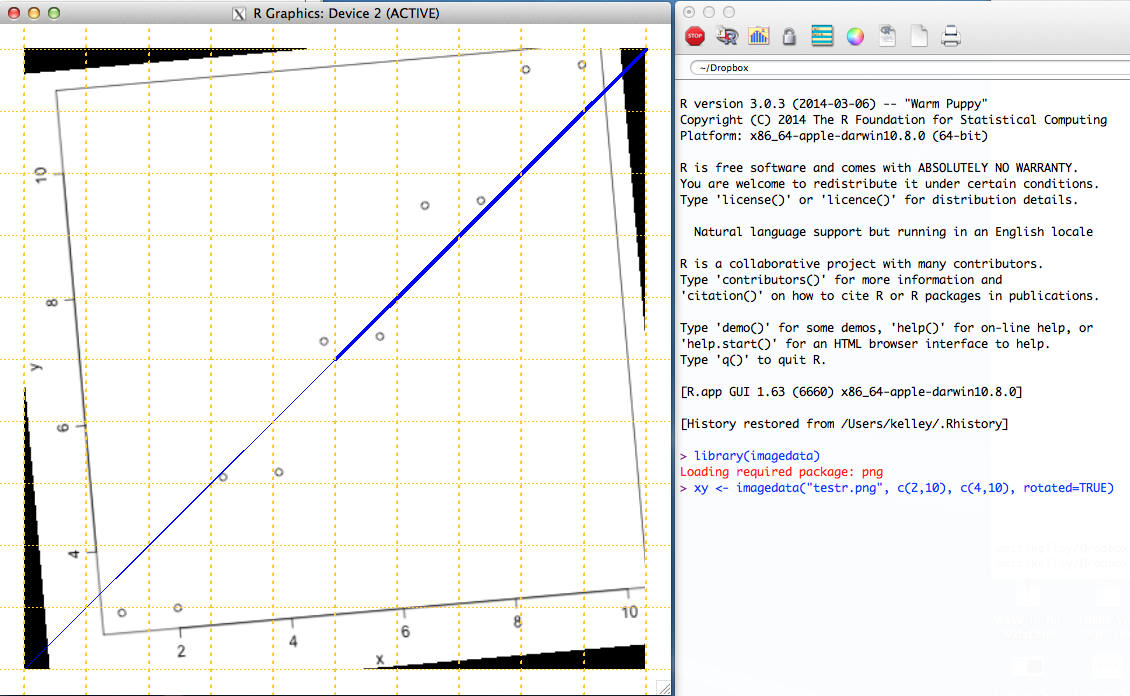
\includegraphics[width=0.5\hsize]{1.png}\end{center}
    \caption{\label{f:rotation}The image-rotation window.}
\end{figure}

If the \texttt{rotated} argument to \function{imagedata} is set to \code{TRUE},
the first window shown to the user will look something like
Figure~\ref{f:rotation}.  As indicated in the Figure, messages appear in the
console, indicating the expected user action.  Once correction for rotation is
complete, processing occurs as follows.

\begin{figure}[ht]
    \begin{center}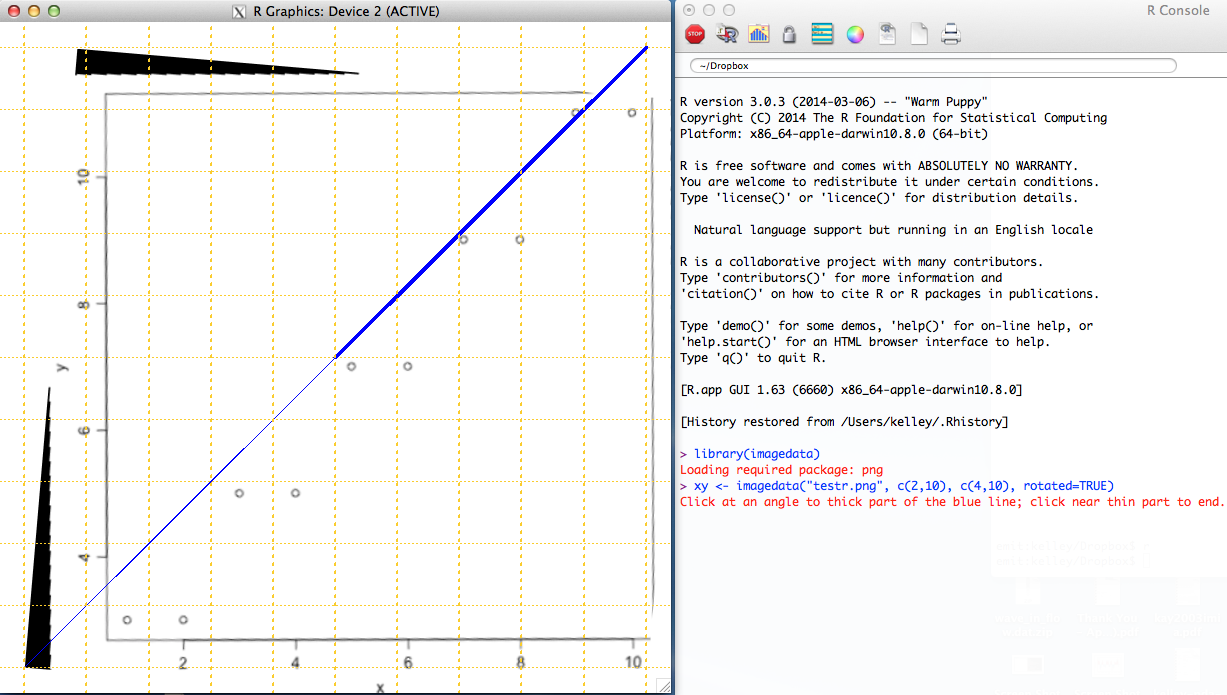
\includegraphics[width=.5\hsize]{2.png}\end{center}
    \caption{\label{f:digitization}The digitization window, showing a case
    with 3 points (red dots) have been digitized.  The user was sloppy, and
    should have clicked in the amber-coloured \code{UNDO} region after clicking the
    point at $x=2$.}
\end{figure}

The user is first invited to click at the lower-left edge of what will become a
\code{UNDO} region.  This should not intersect a part of the plot that has data.
Once the click is made, a coloured box will be drawn, with the word \code{UNDO}
in it.  A similar procedure yields a \code{STOP} region at the top-right of the
image.  Next, the user is invited to click along the $x$ and $y$ axes, at
locations specified by the second and third arguments to \function{imagedata}.
Corrections may be made by clicking \code{UNDO}.  The process is ended when the
user clicks \code{STOP}.  Figure~\ref{f:digitization} illustrates this
procedure.

To add data for a second curve, use \function{getdata}, supplying it with some
arguments that were returned by a previous call to \function{imagedata}.  This
is all explained in the documentation.



\end{document}
